\documentclass[a4paper,12pt]{article}
\usepackage[utf8]{inputenc}
\usepackage[czech]{babel}
\usepackage[T1]{fontenc}
\usepackage{graphicx}
\usepackage{array}
\usepackage{booktabs}
\usepackage{tabularx}
\usepackage{makecell}
\usepackage{float}
\usepackage{url}
\usepackage{listings}
\usepackage{xcolor}
\usepackage{diagbox}
\usepackage{hyperref}
\newcommand{\centered}[1]{\begin{tabular}{l} #1 \end{tabular}}
\newcommand{\unit}[1]{\ensuremath{\, \mathrm{#1}}}
\addto\captionsczech{\renewcommand{\refname}{Seznam použité literatury}}
\addto\captionsczech{\renewcommand{\figurename}{\textbf{Obrázek}}}
\addto\captionsczech{\renewcommand{\tablename}{\textbf{Tabulka}}}
\renewcommand{\lstlistingname}{\textbf{Kód}}

\lstset{
    language=Python,
    basicstyle=\ttfamily\footnotesize,  % Zmenšené písmo
    keywordstyle=\color{blue},
    commentstyle=\color{gray},
    stringstyle=\color{red},
    numbers=left,
    numberstyle=\tiny\color{gray},
    stepnumber=1,
    breaklines=true,
    frame=single
}

\begin{document}
\vspace{\fill}
\begin{center}
    \renewcommand{\arraystretch}{1.75}
    \begin{tabularx}{\textwidth}{|X|X|X|}
        \hline
        \multicolumn{1}{|c|}{\rule{0pt}{2.25cm} 
\includegraphics[height=2cm]{img/ctu_logo.png}} & 
        \multicolumn{2}{c|}{\makecell{\textbf{KATEDRA FYZIKY}}} \\
        \hline
        \multicolumn{3}{|c|}{\Large \textbf{\centered{LABORATORNÍ CVIČENÍ Z FYZIKY}}} \\
        \hline
        \multicolumn{2}{|X}{\small{Jméno} \newline \textbf{Pavel Pernička}} & \multicolumn{1}{|X|}{\small{Datum měření} \newline \textbf{3.4.2025}} \\
        \hline
        {\small{Semestr} \newline \textbf{Letní 2025}} & {\small{Ročník} \newline \textbf{1.}} & {\small{Datum odevzdání} \newline \textbf{17.4.2025}} \\
        \hline
        {\small{Stud. skupina} \newline \textbf{6}} & {\small{Lab. skupina} \newline \textbf{1031}} & {\small{Klasifikace} \newline}\\
        \hline
        \multicolumn{3}{|c|}{\rule{0pt}{1cm}} \\
        \hline
        \multicolumn{1}{|X|}{\small{Číslo úlohy \newline \textbf{7}}} &
        \multicolumn{2}{|p{7cm}|}{\small{Název úlohy \newline \textbf{Měření síly působící na proudovodič}}} \\

        \hline
    \end{tabularx}
\end{center}

\newpage

\section{Úkol měření}
Prozkoumejte závislost mezi proudem protékajícím vodičem v magnetickém poli a silou, jež na
vodič působí.

\section{Seznam použitých přístrojů}
\begin{itemize}
    \item 2x Ručičkový ampérmetr
        \begin{itemize}
        \item Třída přesnosti: $1,5$
        \item Rozsah pro měření $I_m$: $0-1$ A
        \item Rozsah pro měření $I_L$: $0-5$ A
    \end{itemize}
    \item Zdroj
        \begin{itemize}
        \item DC výstup: $0-18$ V, $0-5$ A
        \item AC výstup: $2-15$ V, $5$ A max
    \end{itemize}
    \item Mechanická laboratorní váha
        \begin{itemize}
        \item Nejmenší dílek stupnice: $0,01$ g
    \end{itemize}
    \item Proudovodičové smyčky
        \begin{itemize}
        \item $l=12,5$ mm, 1 závit
        \item $l=25$ mm, 1 závit
        \item $l=50$ mm, 1 závit
        \item $l=50$ mm, 2 závity (budeme používat označení $l=100$ mm)
    \end{itemize}
    \item Elektromagnet
    \begin{itemize}
        \item $I_{max} = 1,3$ A
        \item $R = 6$ $\Omega$
        \item $L = 24$ mH
        \item Podkovovité železné jádro se vzduchovou mezerou $d=10$ mm
    \end{itemize}
    \item Usměrňovací můstek
    \item Závěsné vodiče pro proudovodičové smyčky
\end{itemize}
\section{Měření}
\subsection{Postup}
\begin{enumerate}
    \item Provedeme kontrolu měřicí aparatury a uvedeme ji do výchozího stavu. Ujistíme se, že v tuto chvíli neteče proud obvodem proudové smyčky, ani obvodem elektromagnetu.
    \item Zvolíme jednu z proudových smyček a zavěsíme ji na rameno váhy. Připojíme kontakty ze zavěšeného vodiče.
    \item Pomocí posouvání závažíčka a otáčení vyvažovacího kolečka vyrovnáme rameno váhy a~poznamenáme si tento stav pro pozdější využití pro přepočet na sílu působící na vodič.
    \item Spínačem pustíme proud do obou obvodů a pozorujeme vychýlení váhy. Pomocí kolečka uvedeme váhu zpět do rovnovážného stavu a odečteme hodnotu.
    \item Provedeme body 3 a 4 pro pět různých nastavení proudu, co protéká  proudovou smyčkou ($I_L$), přičemž při každém nastavení $I_L$ provedeme pět dalších měření s různým nastavením $I_m$. Proud $I_L$ volíme v rozsahu $[1;5]$ A, proud $I_m$ volíme nepřímo pomocí napěťového konfigurátoru na zdroji, abychom dostali proud v rozsahu $[0,2;0,9]$ A. Volbu proudů $I_m$ pro každou iteraci se zvoleným proudem $I_L$ necháme vždy stejnou.
    \item Pevně nastavíme $I_L$ spolu s $I_m$ a pomocí stejné metody nepřímo změříme síly při volbě různých proudovodičových přípravků.
\end{enumerate}

\subsection{Naměřené hodnoty}
Pro různá nastavení proudu jsme naměřili pomocí váhy hmotnosti (Tabulky~\ref{tab:l25}, \ref{tab:l50}), od kterých nejprve odečteme hmotnost při nulovém protékajícím proudu $m_0$, abychom získali váhovou výchylku. Z té následně vypočítáme výslednou sílu pomocí vztahu:
$$
F = (m - m_0) \cdot g\ [N],\quad g=9,81\ m \cdot s^{-2},\quad m_{025} = 33,42\ g,\quad m_{050} = 38,72\ g
$$

Výsledek je znázorněn tabulkami \ref{tab:sila25}, \ref{tab:sila50}. Dále jsme provedli měření při konstantním $I_L$ a $I_m$ s různými proudovými smyčkami. Ta byla zpracována obdobným způsobem a jsou znázorněna tabulkou \ref{tab:sila_vs_delka_horizontal}.

\begin{table}[H]
    \centering
    \renewcommand{\arraystretch}{1.5}
    \begin{tabular}{|c|c|c|c|c|c|}
        \hline
        \scriptsize\diagbox[width=6em,height=3.2em]{$\mathbf{I_L}$}{\smash{\raisebox{-1ex}{\scriptsize$\mathbf{I_m}$}}} 
        & \textbf{0,20 A} & \textbf{0,38 A} & \textbf{0,54 A} & \textbf{0,72 A} & \textbf{0,90 A} \\ \hline
        \textbf{1 A} & 33,43 g & 33,53 g & 33,67 g & 33,74 g & 33,84 g \\ \hline
        \textbf{2 A} & 33,60 g & 33,80 g & 34,00 g & 34,16 g & 34,35 g \\ \hline
        \textbf{3 A} & 33,70 g & 34,00 g & 34,27 g & 34,60 g & 34,85 g \\ \hline
        \textbf{4 A} & 33,81 g & 34,20 g & 34,55 g & 34,93 g & 35,33 g \\ \hline
        \textbf{5 A} & 33,93 g & 34,41 g & 34,87 g & 35,41 g & 35,80 g \\ \hline
    \end{tabular}
    \caption{Naměřené hodnoty pro smyčku délky $l = 25$ mm}
    \label{tab:l25}
\end{table}

\begin{table}[H]
    \centering
    \renewcommand{\arraystretch}{1.5}
    \begin{tabular}{|c|c|c|c|c|c|}
        \hline
        \scriptsize\diagbox[width=6em,height=3.2em]{$\mathbf{I_L}$}{\smash{\raisebox{-1ex}{\scriptsize$\mathbf{I_m}$}}} 
        & \textbf{0,20 A} & \textbf{0,38 A} & \textbf{0,54 A} & \textbf{0,72 A} & \textbf{0,90 A} \\ \hline
        \textbf{1 A} & 38,97 g & 39,13 g & 39,33 g & 39,50 g & 39,67 g \\ \hline
        \textbf{2 A} & 39,20 g & 39,54 g & 39,90 g & 40,24 g & 40,57 g \\ \hline
        \textbf{3 A} & 39,40 g & 39,92 g & 40,47 g & 41,00 g & 41,42 g \\ \hline
        \textbf{4 A} & 39,67 g & 40,33 g & 41,02 g & 41,73 g & 42,30 g \\ \hline
        \textbf{5 A} & 39,89 g & 40,70 g & 41,52 g & 42,42 g & 43,21 g \\ \hline
    \end{tabular}
    \caption{Naměřené hodnoty pro smyčku délky $l = 50$ mm}
    \label{tab:l50}
\end{table}

\begin{table}[H]
    \centering
    \renewcommand{\arraystretch}{1.5}
    \begin{tabular}{|c|c|c|c|c|c|}
        \hline
        \scriptsize\diagbox[width=6em,height=3.2em]{$\mathbf{I_L}$}{\smash{\raisebox{-1ex}{\scriptsize$\mathbf{I_m}$}}} 
        & \textbf{0,20 A} & \textbf{0,38 A} & \textbf{0,54 A} & \textbf{0,72 A} & \textbf{0,90 A} \\ \hline
        \textbf{1 A} & 0,10 mN & 1,08 mN & 2,45 mN & 3,14 mN & 4,12 mN \\ \hline
        \textbf{2 A} & 1,77 mN & 3,73 mN & 5,69 mN & 7,26 mN & 9,12 mN \\ \hline
        \textbf{3 A} & 2,75 mN & 5,69 mN & 8,34 mN & 11,58 mN & 14,03 mN \\ \hline
        \textbf{4 A} & 3,83 mN & 7,65 mN & 11,09 mN & 14,81 mN & 18,74 mN \\ \hline
        \textbf{5 A} & 5,00 mN & 9,71 mN & 14,22 mN & 19,52 mN & 23,35 mN \\ \hline
    \end{tabular}
    \caption{Spočítané síly pro délku smyčky $l = 25$ mm}
    \label{tab:sila25}
\end{table}

\begin{table}[H]
    \centering
    \renewcommand{\arraystretch}{1.5}
    \begin{tabular}{|c|c|c|c|c|c|}
        \hline
        \scriptsize\diagbox[width=6em,height=3.2em]{$\mathbf{I_L}$}{\smash{\raisebox{-1ex}{\scriptsize$\mathbf{I_m}$}}} 
        & \textbf{0,20 A} & \textbf{0,38 A} & \textbf{0,54 A} & \textbf{0,72 A} & \textbf{0,90 A} \\ \hline
        \textbf{1 A} & 2,45 mN & 4,02 mN & 5,98 mN & 7,65 mN & 9,32 mN \\ \hline
        \textbf{2 A} & 4,71 mN & 8,04 mN & 11,58 mN & 14,91 mN & 18,15 mN \\ \hline
        \textbf{3 A} & 6,67 mN & 11,77 mN & 17,17 mN & 22,37 mN & 26,49 mN \\ \hline
        \textbf{4 A} & 9,32 mN & 15,79 mN & 22,56 mN & 29,53 mN & 35,12 mN \\ \hline
        \textbf{5 A} & 11,48 mN & 19,42 mN & 27,47 mN & 36,30 mN & 44,05 mN \\ \hline
    \end{tabular}
    \caption{Spočítané síly pro délku smyčky $l = 50$ mm}
    \label{tab:sila50}
\end{table}

\begin{table}[H]
    \centering
    \renewcommand{\arraystretch}{1.4}
    \begin{tabular}{|l|c|c|c|c|}
        \hline
        \textbf{Délka} $l$ \textbf{[mm]} & 12,5 & 25 & 50 & 100 \\ \hline
        \textbf{Síla} $F$ \textbf{[mN]} & 8,44 & 14,81 & 29,53 & 54,25 \\ \hline
    \end{tabular}
    \caption{Závislost síly na délce smyčky pro $I_m = 0{,}9\,\mathrm{A}$ a $I_l = 3\,\mathrm{A}$}
    \label{tab:sila_vs_delka_horizontal}
\end{table}

\section{Výpočty}
Abychom potvrdili naše výsledky, srovnáme naměřené síly s teoreticky vypočítanými silami podle vzorce:
$$
F = B \cdot I_L \cdot l
$$
Srovnání provedeme na datech závislost síly na délce smyčky z tabulky \ref{tab:sila_vs_delka_horizontal} a~ukážeme v tabulce \ref{tab:sila_vs_delka_theory}. Druhé srovnání provedeme na datech závislosti síly na proudu $I_m$ při $I_L = 1\ A$ a $l=50\ mm$ v prvním řádku tabulky \ref{tab:sila50}.

Vzhledem k tomu, že magnetické pole je kolmé na proud protékaný smyčkou a známe magnetickou indukci $B_0 = 168\ mT$ při $I_m = 0,87\ A$, z přímé úměry můžeme vypočítat $B$ při všech měřených proudech $I_m$. Tento převod je dán tabulkou \ref{tab:convert}. 

\begin{table}[H]
    \centering
    \renewcommand{\arraystretch}{1.4}
    \begin{tabular}{|l|c|c|c|c|c|}
        \hline
        \textbf{Proud} $I_m$ \textbf{[A]} & 0,2 & 0,38 & 0,54 & 0,72 & 0,90 \\ \hline
        \textbf{Indukce} $B$ \textbf{[mT]} & 38,62 & 73,38 & 104,28 & 139,03 & 173,79 \\ \hline
    \end{tabular}
    \caption{Vypočtená magnetická indukce pro jednotlivé proudy $I_m$}
    \label{tab:convert}
\end{table}

\begin{table}[H]
    \centering
    \renewcommand{\arraystretch}{1.4}
    \begin{tabular}{|l|c|c|c|c|}
        \hline
        \textbf{Délka} $l$ \textbf{[mm]} & 12,5 & 25 & 50 & 100 \\ \hline
        \textbf{Síla} $F$ \textbf{[mN]} & 6,52 & 13,03 & 26,07 & 52,14 \\ \hline
    \end{tabular}
    \caption{Teoretická síla pro jednotlivé délky smyčky za proudů $I_m = 0{,}9\,\mathrm{A}$ (tedy $B=$) a $I_l = 3\,\mathrm{A}$}
    \label{tab:sila_vs_delka_theory}
\end{table}

\begin{table}[H]
    \centering
    \renewcommand{\arraystretch}{1.4}
    \begin{tabular}{|l|c|c|c|c|c|}
        \hline
        \textbf{Proud} $I_m$ \textbf{[A]} & 0,2 & 0,38 & 0,54 & 0,72 & 0,90 \\ \hline
        \textbf{Indukce} $B$ \textbf{[mT]} & 38,62 & 73,38 & 104,28 & 139,03 & 173,79 \\ \hline
        \textbf{Síla} $F$ \textbf{[mN]} & 1,93 & 3,67 & 5,21 & 6,95 & 8,69 \\ \hline
    \end{tabular}
    \caption{Teoretická síla pro smyčku $l=50\ mm$ při proudu $I_L=1\ A$}
    \label{tab:sila_vs_Im_theory}
\end{table}

\section{Grafy}
Abychom ukázali linearitu závislosti naměřených veličin k sobě navzájem, vykreslili jsme je do grafů -- graf \ref{fig:F_vs_Il} ukazuje závislost naměřené síly na proudu $I_L$, graf \ref{fig:F_vs_Im} závislost síly na magnetizačním proudu $I_m$. Naměřenými body byla proložena přímka pomocí metody nejmenších čtverců. 

Obdobným způsobem je zpracována závislost síly na délce proudovodičové smyčky v grafu \ref{fig:F_vs_l_measured_theory}. Zde je vykreslena i teoretická síla vypočítaná v předchozí sekci v tabulce \ref{tab:sila_vs_delka_theory}. Stejně jsme srovnali naměřenou sílu při měnící se $I_m$ s~teoretickými hodnotami v grafu \ref{fig:F_vs_Im_theory_single}.

U obou grafů s porovnáním můžeme vidět, že směrnice proložené přímky a přímky teoretických sil jsou téměř stejné, tedy datové série se navzájem liší jen o konstantu.

\begin{figure}[H]
    \centering
    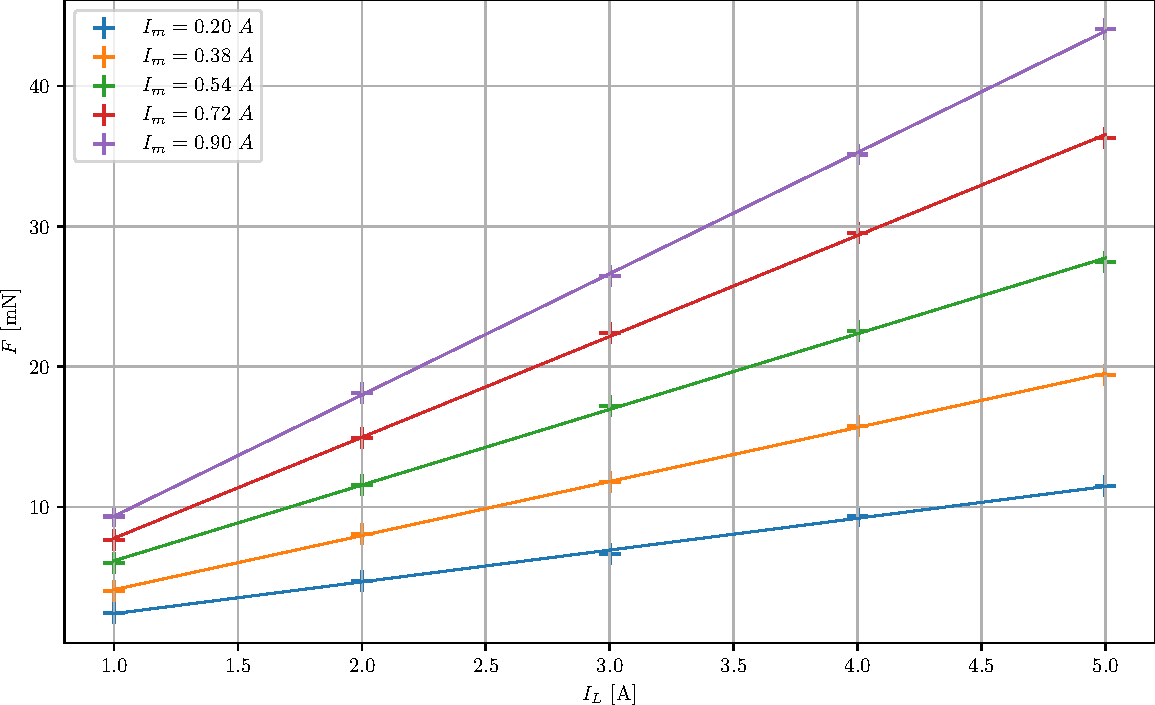
\includegraphics[width=1\textwidth]{img/F_vs_Il.pdf}
    \caption{Závislost síly $F$ na $I_L$ při $l=50\ mm$}
    \label{fig:F_vs_Il}
\end{figure}

\begin{figure}[H]
    \centering
    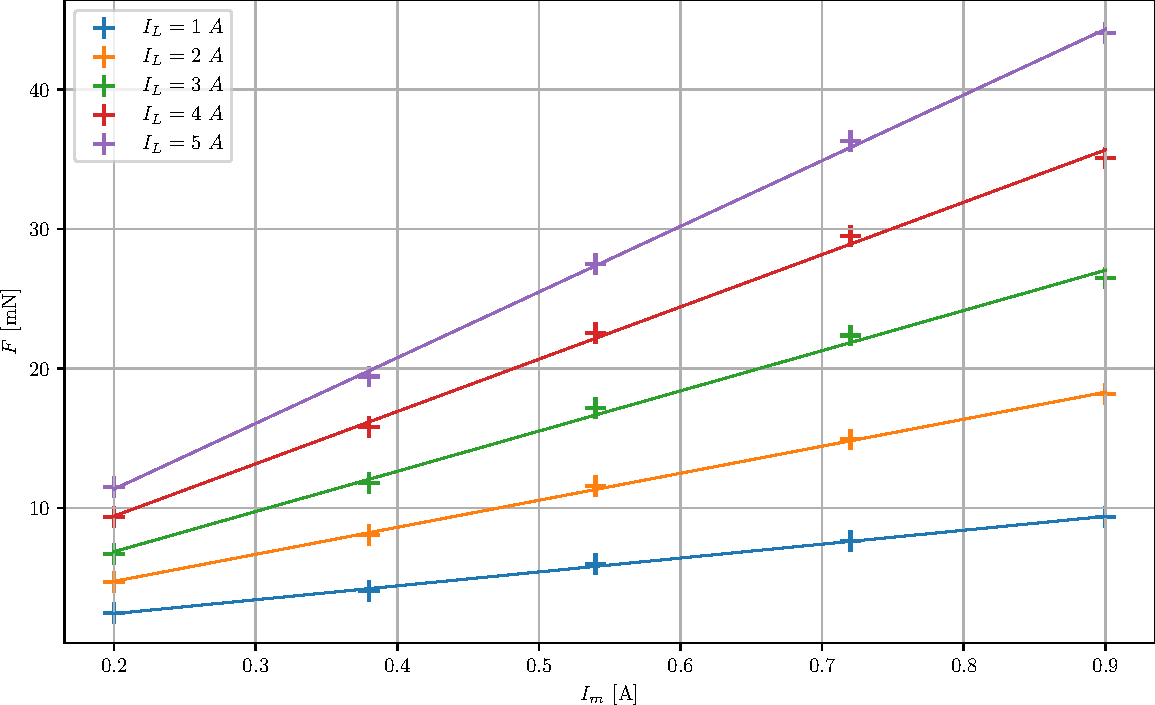
\includegraphics[width=1\textwidth]{img/F_vs_Im.pdf}
    \caption{Závislost síly $F$ na $I_m$ při $l=50\ mm$}
    \label{fig:F_vs_Im}
\end{figure}

\begin{figure}[H]
    \centering
    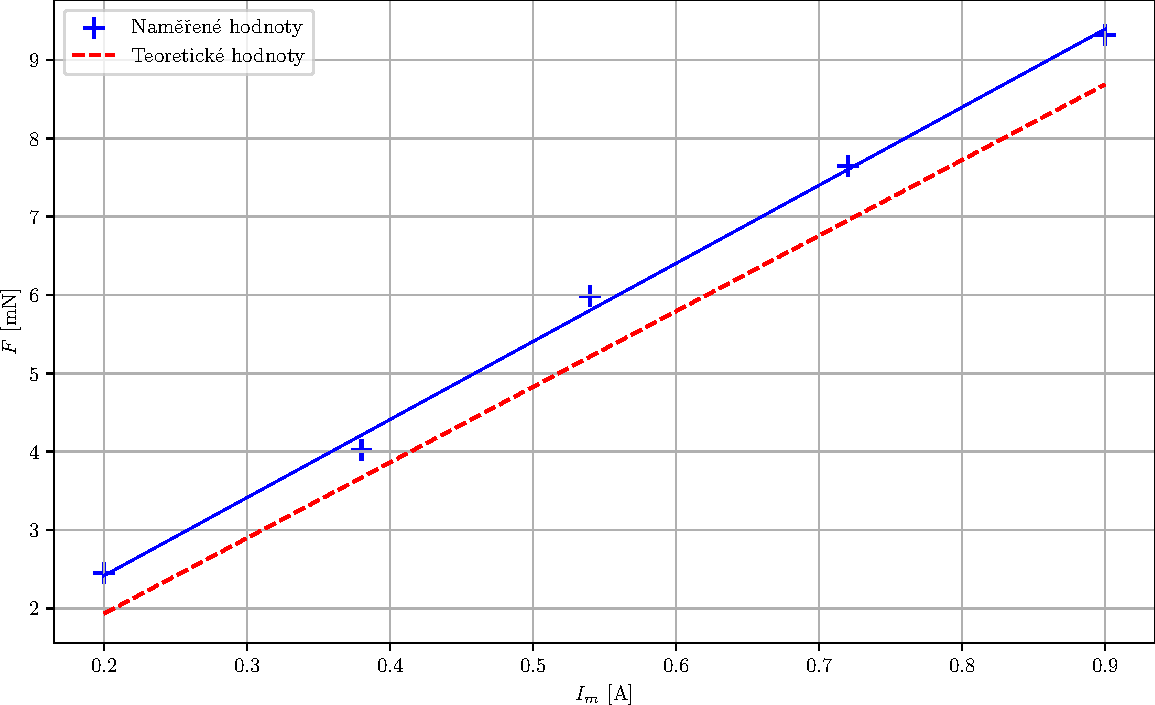
\includegraphics[width=1\textwidth]{img/F_vs_Im_theory_single.pdf}
    \caption{Srovnání závislost síly $F$ na $I_m$ ($I_L=1\ A$, $l=50\ mm$) s~teoretickými hodnotami}
    \label{fig:F_vs_Im_theory_single}
\end{figure}

\begin{figure}[H]
    \centering
    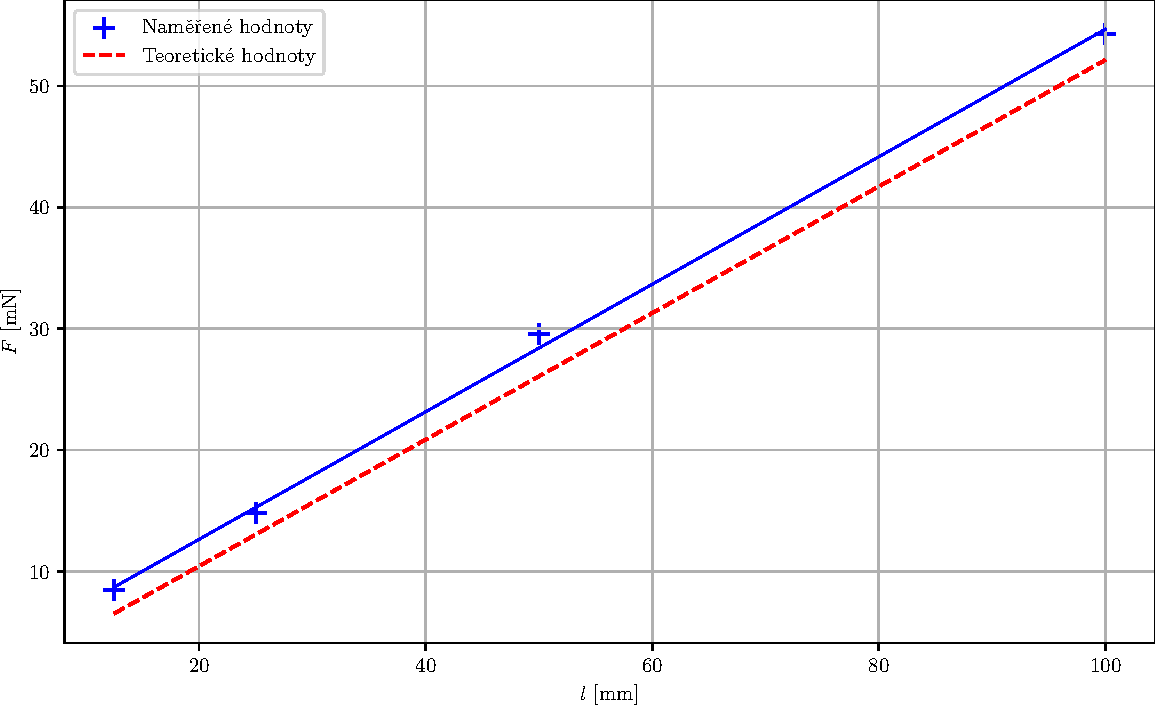
\includegraphics[width=1\textwidth]{img/F_vs_l_measured_theory.pdf}
    \caption{Srovnání závislosti síly $F$ na délce $l$ ($I_m=0,90\ A$, $I_L=3\ A$) s~teoretickými hodnotami}
    \label{fig:F_vs_l_measured_theory}
\end{figure}

\section{Nejistoty}
Prvotní nejistota, kterou bychom měli zahrnout, je standardní nejistota typu B -- $u_B$, která pochází z nepřesnosti použitých měřicích přístrojů a je dána vztahem:
$$
u_B = \frac{2\cdot R \cdot (TP/100)}{\sqrt{12}}
$$
kde $R$ je rozsah přístroje a $TP$ je třída přesnosti přístroje. Pro váhu použijeme jen vztah:
$$
u_B = \frac{\Delta}{\sqrt{12}}
$$
kde $\Delta$ je velikost nejmenšího dílku na stupnici.
Pomocí těchto vztahů můžeme postupně vyjádřit $u_B$ pro jednotlivá zařízení: laboratorní váhy a~ampérmetry pro měření $I_m$ a $I_L$:
$$
u_B(m) = \frac{0,01}{\sqrt{12}}=0,0029\ g
$$
$$
u_B(I_m) = \frac{2\cdot (1,5/100)}{\sqrt{12}} = 0,0086\ A
\quad
u_B(I_L) = \frac{10\cdot (1,5/100)}{\sqrt{12}} = 0,0433\ A
$$

Dále pak jsme schopni vyjádřit nepřesnost našeho měření pomocí proložení přímky našimi daty. K~tomuto účelu využijeme tabulku \ref{tab:l50} a polynom získaný při tvorbě grafu, pomocí něhož vypočítáme střední kvadratickou odchylku námi naměřených od hodnot na proložené přímce. Toto provedeme pro závislost $F$ na $I_m$ a pro $F$ na $I_L$ zvlášť podle vzorce:
$$
\delta = \sqrt{ \frac{1}{n} \sum_{i=1}^{n} \left( y_i - \hat{y}_i \right)^2 }
$$
kde $y_i$ jsou naměřené hodnoty, $\hat{y}_i$ jsou hodnoty z proložené přímky a $n$ je počet bodů. 

Z odchylek pro oboje závislosti dále vypočítáme celkovou odchylku pomocí vztahu ($m$ a $n$ jsou počty měření jednotlivých proudů):
$$
\delta_{ALL} = \sqrt{ \frac{1}{2} \left( \frac{1}{m} \sum_{i=1}^{m} \delta(I_m)_i^2 + \frac{1}{n} \sum_{j=1}^{n} \delta(I_L)_j^2 \right) }
$$

Pomocí výpočetního skriptu v jazyce Python získáváme hodnotu:
$$
\delta_{ALL} = 0,252\ mN
$$
\section{Závěr}
Fyzikální teorie předpokládá, že velikost síly $F$ působící na proudovodič v~homogenním magnetickém poli je přímo úměrná délce vodiče $l$, velikosti magnetické indukce $B$ (resp. magnetizačnímu proudu $I_m$) a velikosti proudu \( I_L \) protékajícího vodičem, tedy že platí vztah:
$$
F = B\cdot I_L\cdot l
$$

Na základě experimentálních dat lze tuto závislost potvrdit. Závislost síly na všech třech proměnných byla ověřena pomocí několika měření a grafů, které prokázaly téměř lineární průběh. Výsledky měření vzhledem k malé odchylce $\delta_{ALL}$ od proložených přímek odpovídají teoretickému předpokladu.

Mezi pravděpodobné zdroje nepřesností patří:
\begin{itemize}
    \item nepřesný odečet z vah způsobený např. rozkmitem,
    \item fakt, že magnetické pole není i při malé vzdálenosti zcela homogenní,
    \item nepřesnosti v konstrukci měřicí aparatury, např. nesymetrické zavěšení smyčky a hmotnost napájecích vodičů k ní),
    \item nedokonalé vyvážení při kalibraci váhy na začátku měření (lze vidět jako posun přímky o konstantu na porovnání s vypočtenými silami v~grafech \ref{fig:F_vs_Im_theory_single} a~\ref{fig:F_vs_l_measured_theory}).
\end{itemize}


\begin{thebibliography}{}

    \bibitem{perm}
    Milan Červenka, Karel Malinský. \textit{Měření síly působící na proudovodič}. Laboratorní úloha, 2013. Dostupné online: \url{https://planck.fel.cvut.cz/praktikum/downloads/navody/proudovahy.pdf}.

    \bibitem{zpracdat}
    Milan Červenka. \textit{Zpracování fyzikálních měření}. Studijní text pro fyzikální praktikum, 2020. Dostupné online: \url{https://planck.fel.cvut.cz/praktikum/downloads/navody/zpracdat.pdf}.

\end{thebibliography}

\end{document}
